% THIS IS SIGPROC-SP.TEX - VERSION 3.1
% WORKS WITH V3.2SP OF ACM_PROC_ARTICLE-SP.CLS
% APRIL 2009

\documentclass{acm_proc_article-sp}

\begin{document}

\title{ Expresso: Typesetting Handwritten Mathematical Expressions on the Post-PC Tablet Computer }
\subtitle{ [Project Final Report] }

\numberofauthors{2} 

\author{
\alignauthor
Josef Lange\\
       \affaddr{University of Puget Sound}\\
       \affaddr{1130 NW 54th St \#617S}\\
       \affaddr{Seattle, WA 98107}\\
       \email{josef.d.lange@me.com}
\alignauthor       
Daniel Guilak\\
       \affaddr{University of Puget Sound}\\
       \affaddr{3396 Wheelock Student Center}\\
       \affaddr{Tacoma, WA 98416-3396}\\
       \email{dguilak@pugetsound.edu}
}
       
\date{20 April, 2013}

\maketitle

\begin{abstract}
This paper sets forth to describe our process and products of fulfilling the capstone requirement of the Bachelor's Degree in Computer Science at the University of Puget Sound. Our project was to research, design, and implement a tablet-based software solution for the capture of handwritten mathematical expressions and compilation of its mathematical representation into an appropriate representative language (such as \LaTeX or MathML).

Subjects approached in our project include image processing, artificial intelligence, application development for the Apple iOS platform (particularly in the tablet form factor), server development, as well as the adherence to a highly disciplined development cycle. We will attempt to most accurately and most briefly explain any uncommon concepts described hereafter.
\end{abstract}

\section{Introduction}
The utility of the touch-based computer interaction has only been recently fully realized, with the nascence of the ``Post-PC'' tablet in its migration away from the standard desktop usage paradigm commonly associated with computing. The modern tablet focuses on media consumption and so-called ``basic'' computing. In today's reality, most ``Post-PC'' tablets are incredibly powerful both in hardware and in software, supporting complex and challenging computations including the decoding of video, image processing, interpretation of multiple inputs, managing several network connections, and displaying high-resolution two- and three-dimensional graphics. Past their technical capabilities, these small computers have found their way into near-ubiquity of use. 

The touch interface of a ``Post-PC'' tablet offers a unique tool to any consumer---the direct input of figures via touch---that has only previously been common to graphics and imaging professionals. Expresso sets out to take advantage of this new ubiquity in direct-interaction computing by positioning itself as an alternate input method for document production.

\section{Related Work}

\subsection{General Handwriting Recognition} 
Handwriting recognition is a complex problem, only a segment of which my project wishes to solve. Existing solutions to handwriting recognition exist, and some  perform at a useable level. Frequently, these systems require a period of ``training'' before any recognition can be achieved. Others use artificial intelligence to conclude what a sequence of handwriting is meant to be. For full-on text recognition, this is useful and almost required for any success. Commercial products exist, including but not limited to software built into Microsoft's Windows and Apple's Mac OS X Operating Systems. Additionally, many third-party companies have produced software for a similar purpose.

\subsection{Mathematical Expression Capture}
General handwriting recognition solutions are frequently overpowered for the niche of mathematical expressions, in which there are fewer possible logical constructs, most of which follow a fairly standard form. Because of this, the subset of things needing recognition, and possibilities for what they could be recognized as, is significantly smaller. Academic projects, including those by Matsakis\cite{matsakis_recognition_1999}, Smithies et. al.\cite{smithies_handwriting-based_1999}, and Levin\cite{levin_cellwriter:_2007} exhibit valid solutions for the desktop model of usage, though are not implemented in a way that is ultimately accessible for the common user.

\section{Proposed Solution}
This project will produce a feature-complete, usable piece of software for the Apple iOS platform. This software will have a singular function: to capture handwritten mathematical expressions via the digitizing screen, and communicate with a server which will compile the interpreted characters into the appropriate mathematical representational language (namely \LaTeX or MathML). 

\section{Motivation \& Importance}
Throughout their history, touch devices have attempted to attain status as a ``universal tool'' -- something able to function seamlessly in their users' lives. Humans communicate naturally with handwriting, and devices from Apple Newtons, to Palm Pilots, to Pocket PCs, and now to the likes of the Apple iPad, Amazon Kindle Fire, and Microsoft Surface have tried to integrate handwriting recognition with little success since software keyboards are more familiar and efficient to most users. However, we believe that the size and shape of tablet devices are reminiscent of ``slates" used in classrooms to scribble out mathematical equations.

Both authors at one point or another have been frustrated with a homework assignments requiring mathematical typesetting in \LaTeX.  We believe it would be great for a user to jot down an equation on an iPad or other tablet device and have the \LaTeX\ code appear on the document they are editing on their laptop or desktop computer.

This software could easily improve the classroom environment in all levels of schooling. Getting mathematical equations into type is a frustrating task for many teachers in the K-12 levels, and even frustrating for the higher-education professor and student. With this software, student and educators alike can easily convert their glyphic mathematical thoughts into usable typesetting language. This will hopefully open doors to clearer and more specific teaching and learning throughout all levels of education.

\section{Method \& Implementation}

\subsection{Overview}
The software components of this project stand upon a foundation of three central parts. See Figure~\ref{fig:final_chart} for a graphical representation of the basic organization. The primary and most visible component is the client application, with which the user (obviously) directly interacts. PLEASE ADD MORE HERE I JUST STARTED TO SEE WHAT IT WOULD LOOK LIKE WITH THE GRAPHIC AND WHATNOT.



\subsection{``Expresso'' (iOS Client)}
The iOS client for Expresso is the face of its distributed computation system. The user directly interacts with Expresso on his or her iPad, iPhone, or iPod touch, and is able to interact with each step of the recognition and identification process. The application itself was developed using Apple's Xcode IDE, freely available to any who wish to develop apps. 

The programming language most commonly used when developing iOS applications is Objective-C, a superset of ANSI C that gives a solid syntax for object-oriented programming. This syntax is a little bizarre at first glance, but is really powerful for rapid development of easily-readable code. 

The availability of first-party frameworks from Apple for developer use is astonishing; if you need to do something you think is more than trivial, chances are there's a class and/or method for that already written. Apple's documentation, too, turned out to be an invaluable tool throughout the development process. 

Even more exciting, and perhaps a bit confusing at first, was the graphical development of a GUI for these apps. While one can programattically lay out an interface for iOS, Xcode includes an Interface Builder, which on-the-fly actually instantiates UI objects and then archives them away when compiling your application, only later to be unarchived and ready-to-go on launch.

iOS development is build upon the foundation of the Model-View-Controller state of mind. Each class should fall into one of these three categories, and there are guidelines as to how members of each category interact. A model class encapsulates data utilized by applications. A view, rather intuitively, is a means by which we see data, whether it is an image view, a table view, a text view, or something like a button. What's left, then, is the controller, the real hard worker of the three categories. A controller is responsible for, to some degree, ``running the show''. Controllers interact with model objects to see and manipulate data. Controllers, too, interact with view objects in order to either change what the view is showing or doing, or to receive information pertaining to user interaction.

\begin{figure*}
\centering
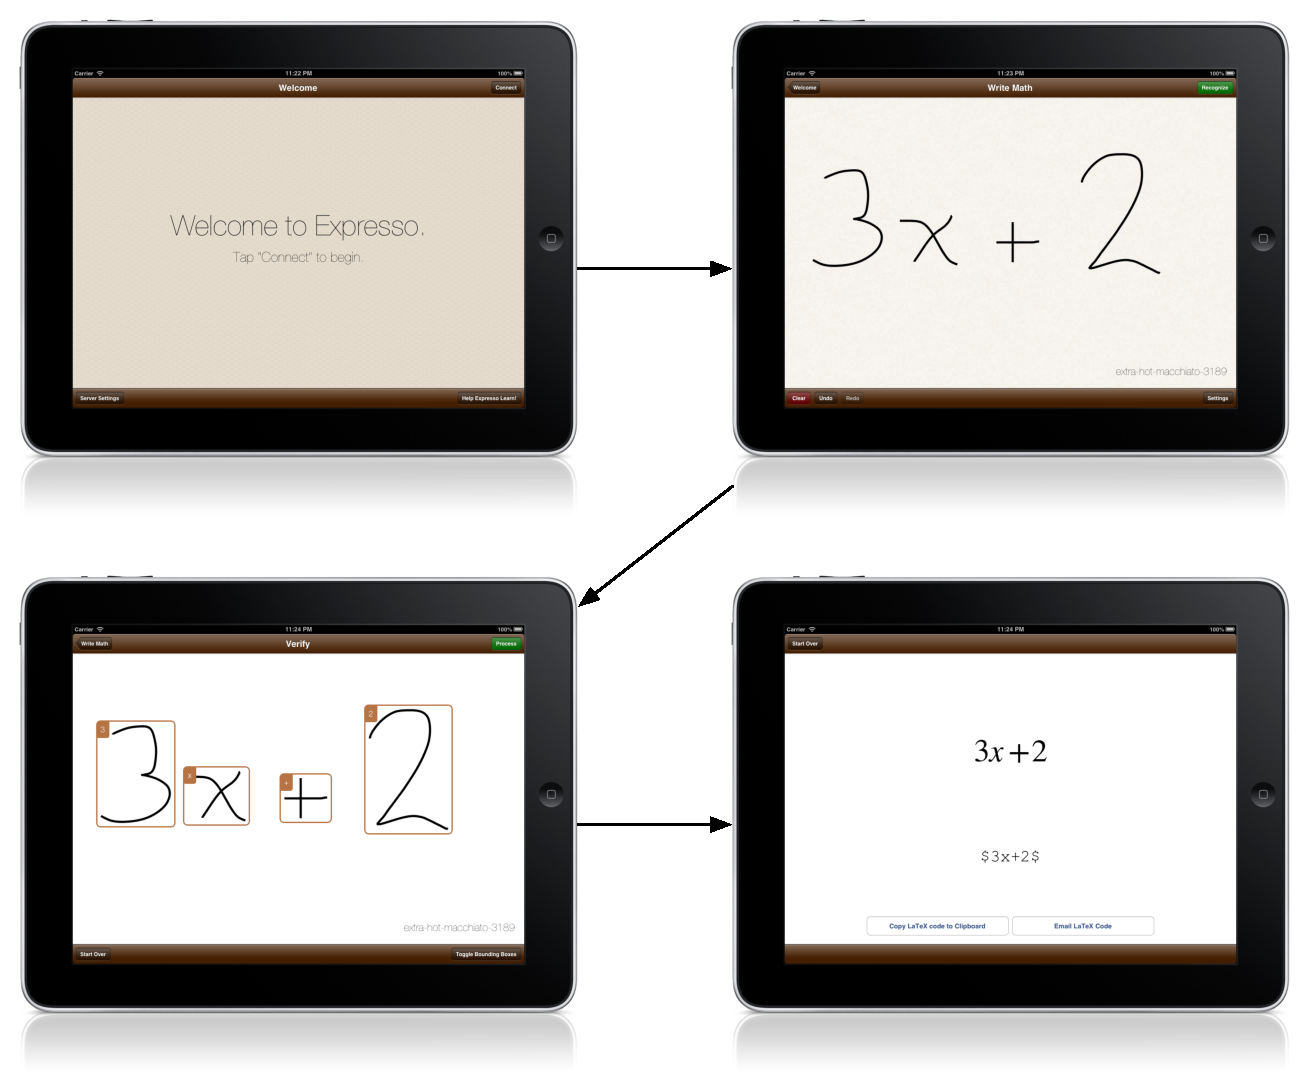
\includegraphics[width=1.0\textwidth]{user_workflow.pdf}
\caption{General User Interaction with Expresso. The user first connects to the web application. Then, they draw their math and send it off. The server returns to the client the recognized symbols. At this point, the user has the opportunity to correct any mistakes Barista and Roaster may have made. Finally, the user requests the crunched-out math and \LaTeX code.}
\label{fig:user_workflow}
\end{figure*}

The general user interaction of the most basic use case is outlined in Figure~\ref{fig:user_workflow}. The application makes use of a Navigation Controller, a special type of View Controller that can be best explained as a slide projector. It takes interaction like, ``show the next UI view!'', or ``Go back to the start!''. Naturally, one can dynamically change what the ``next slide'' will be, but the metaphor still stands. As the user completes a portion of the pipelined tasks of connecting, drawing, correcting, and enjoying, the Controller progresses from the current view to the appropriate next view. Behind the scenes, iOS and Apple's already-built-in magic is doing the really hard work of animating everything.

TODO: CURVE APPROX, OPEN-SOURCE CODE USED

\subsection{``Barista''}

\begin{figure*}
\centering
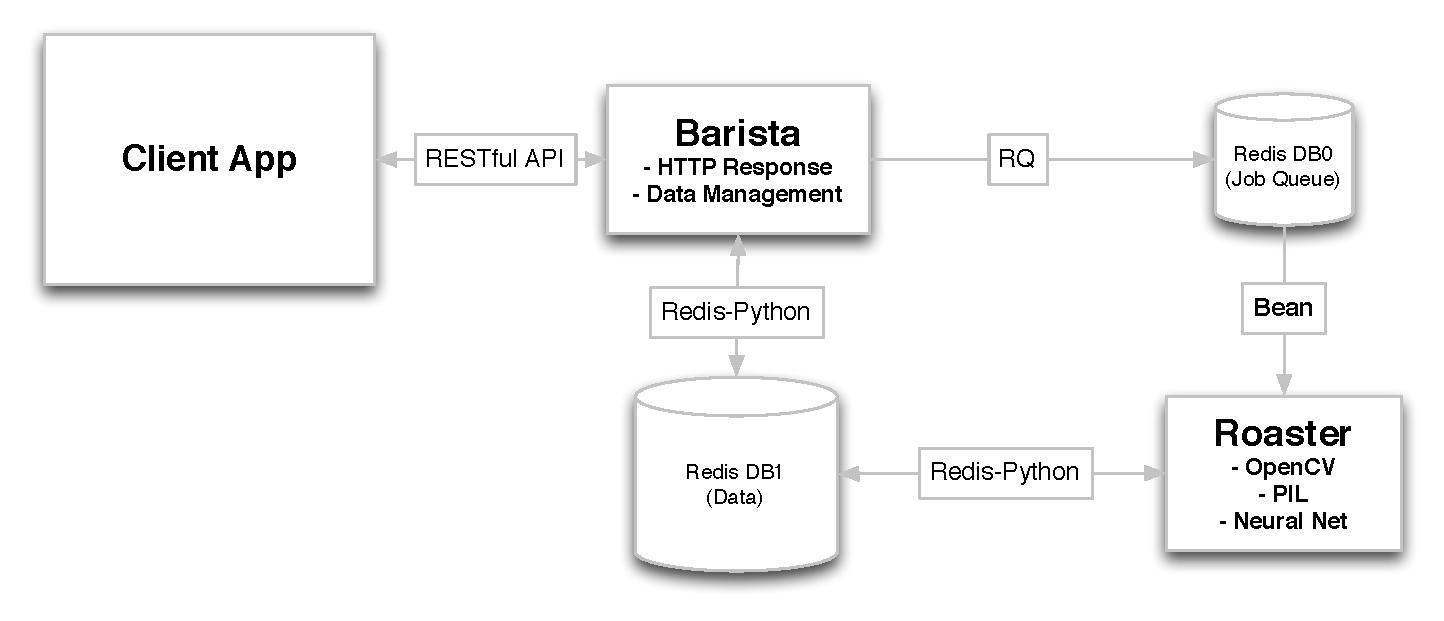
\includegraphics[width=1.0\textwidth]{final_chart.pdf}
\caption{Simplified Organization of Software Components}
\label{fig:final_chart}
\end{figure*}

A barista, in the coffee world, is the person who takes one's coffee order and completes and delivers one's drink. Likewise, Expresso's Barista takes requests for information and delivers said information. The most fitting method of data transmission for our use was that of a RESTful API. REST, or Representational State Transfer, ``relies on a stateless, client-server, cacheable communications protocol''\cite{elkstein_rest_2008}. In essence, REST relies on the fact that no two entities are ever automatically in-sync with one another; an entitie can request data from another and manipulate it, but it must send the updated data back to its source to keep changes consistent across a system. REST has, as of late, become a \emph{de facto} standard amongst software developers looking for a server-client architecture. 

REST is but an idea; there is no official standard to adhere to, nor a strict set of guidelines upon which to build one's API. Fortunately, there exist already-implemented frameworks for the rapid development of REST-minded API server. One such tool is Flask-RESTful\footnote{https://github.com/twilio/flask-restful}, a BSD-licensed Python library that creates a framework for constructing a RESTful API on top of a web server operated by Flask\footnote{http://flask.pocoo.org}. Flask itself is an extremely lightweight web server, also used under the BSD license.

Barista leverages these technologies to serve and receive the data Expresso needs. Of course, every web application software requires web server hardware. For Barista, we selected Heroku\footnote{http://heroku.com}, a mind-shatteringly simple deployment platform for web application software, particularly those programmed in Python or Ruby (we used Python). Launching an application on Heroku is literally as simple as signing up for an account and using Git source control\footnote{http://git-scm.com} to push your code to your account on their servers. Heroku remains free to developers so long as they only run one process at a time. This, of course, presented issues when we wanted to implement recognition functionality modularily, particularly when it looked as though the recognition would need to be running a process of its own. The discussion in Subsection \ref{subsection:roaster} explains our workaround to such an issue.

Barista, since it is a web server, communicates using the HTTP Protocol. In particular, Barista utilizes the GET and POST methods of the HTTP Protocol specification. Their function is rather straighforward; GET requests and expects to receive data, while POST sends and expects the remote updating of data. 

Having an API defined convenient, but what about the data itself? Shouldn't that be represented in some conveniently-standardized manner? That's where JSON\footnote{http://www.json.org} comes in. JSON is a fantastic standardized data format. It supports singular generically-typed elements, and the basic collections of arrays and dictionaries. Utilizing a common vocabulary of keys for requesting values, several different platforms can utilized JSON data without requiring any transformation of the data. Where, then, is the data stored? We ended up utilizing the Redis\footnote{http://redis.io/} NoSQL database system (again BSD-licensed), essentially a very large map of key-value pairs. This allowed us to define our own relationships in code and define and manipulate structures of data on-the-fly. To access Redis, we utilized the Python interface to Redis, redis-py\footnote{https://github.com/andymccurdy/redis-py} (under MIT license).

So, with all this in mind, we designed and developed a two-piece system for Barista. The front-side was essentially a fa\c{c}ade design pattern. It hooked into Flask-RESTful to implement the methods called when certain HTTP requests were made to the server at certain URL paths. Each of these methods utilized the Barista's back-side, a series of classes to Pythonically encapsulate the data stored in the Redis database for our use. Each class has the ability to detect whether or not it is ``dirty'', that is, whether or not the data the object contains is at the same state as its original data in the Redis database. This allows us to instantiate an object from the Barista module, load data into it, manipulate it, and then put the data back. It's almost a RESTful methodology in and of itself.

Barista definitely serves up a mean cup of Expresso.

\subsection{``Roaster'', ``Bean'', \& ``Grinder''}
\label{subsection:roaster}


\section{Evaluation}

\section{Discussion \& Analysis}

\section{Conclusion}

%\end{document}  % This is where a 'short' article might terminate

\bibliographystyle{abbrv}
\bibliography{final_citations}  
% You must have a proper ".bib" file
%  and remember to run:
% latex bibtex latex latex
% to resolve all references
%
% ACM needs 'a single self-contained file'!
%
%APPENDICES are optional
%\balancecolumns


\balancecolumns

% That's all folks!
\end{document}
